%% To submit your paper:
\documentclass[draft]{agujournal2019}
\usepackage{multirow}
\usepackage{url} %this package should fix any errors with URLs in refs.
\usepackage{lineno}
\usepackage[margins,movemargins]{trackchanges} %for better track changes. finalnew  option will compile document with changes incorporated.
\addeditor{Naty}
\addeditor{N}
\addeditor{F}
\addeditor{A}

\usepackage{soul}
\linenumbers

%%%%%%%
% As of 2018 we recommend use of the TrackChanges package to mark revisions.
% The trackchanges package adds five new LaTeX commands:
%
%  \note[editor]{The note}
%  \annote[editor]{Text to annotate}{The note}
%  \add[editor]{Text to add}
%  \remove[editor]{Text to remove}
%  \change[editor]{Text to remove}{Text to add}
%
% complete documentation is here: http://trackchanges.sourceforge.net/
%%%%%%%

\draftfalse

\journalname{Paleoceanography and Paleoclimatology}


\begin{document}


\title{Sensitivity of atmospheric carbon dioxide to dust iron
solubility during the last glacial-interglacial cycle}


% Example: \authors{A. B. Author\affil{1}\thanks{Current address, Antartica}, B. C. Author\affil{2,3}, and D. E.
% Author\affil{3,4}\thanks{Also funded by Monsanto.}}

\authors{N. Opazo\affil{1}, F. Lambert\affil{1}, A. Ridgwell\affil{2}, and N. J. Cosentino\affil{1} }


\affiliation{1}{Instituto de Geografía, Pontificia Universidad Católica de Chile, Santiago, Chile.}
\affiliation{2}{Department of Earth and Planetary Sciences, University of California, Riverside, CA, USA.}

\correspondingauthor{Natalia Opazo}{neopazo@uc.cl}

%Example:
\begin{keypoints}
\item	List up to three key points (at least one is required)
\item	Key Points summarize the main points and conclusions of the article
\item	Each must be 140 characters or fewer with no special characters or punctuation and must be complete sentences
\end{keypoints}


\begin{abstract}
[ enter your Abstract here ]
\end{abstract}

------------------------------------------------------------------------ %%
%
%  TEXT
%
%% ------------------------------------------------------------------------
\section{Introduction}

% !TEX root = ../journaltemplate.tex

Iron (Fe) stands as the fourth most abundant element in the Earth’s crust. Despite its abundance, the concentrations of iron at the oceanic surface remain relatively low, ranging from 0.1 to 2 nM (nanomolar) \cite{nakabayashi2002variation,tani2003iron}. These concentrations have a remarkable impact on the delicate balance of the marine ecosystem. Phytoplankton production, a cornerstone of oceanic food webs and a significant driver of global carbon cycling, can be significantly constrained due to Fe’s crucial enzymatic role \cite{martin1990glacial,jickells2005global,martinez2014iron}. Notably influencing processes like photosynthesis, respiration, and nitrogen fixation \cite{falkowski1998biogeochemical,morel2003biogeochemical,kustka2003revised}, Fe becomes a limiting factor that reverberates through the marine food chain. This influence assumes heightened significance in specific regions, such as the Southern Oceans, the Pacific and North Atlantic, and the Eastern Equatorial Pacific, collectively known as high-nutrient low-chlorophyll concentration (HNLC) zones \cite{coale1996massive,boyd2000mesoscale,boyd2004decline,boyd2007mesoscale}. 

Several pathways contribute to delivering this essential micronutrient to the ocean’s surface. Hydrothermal vents, rivers, glaciers, icebergs, continental edges, and upwelling mechanisms all play roles in introducing iron into oceanic ecosystems \cite{ducklow2003role,tagliabue2016well}. Nevertheless, beyond continental margins, the importance of dust fluxes, sourced from arid and semi-arid desert regions, emerges as a fundamental factor \cite{tagliabue2017integral,lambert2021regional}. These dust fluxes, mobilized by wind forces and sometimes traveling substantial distances, settle onto the ocean surface through dry or wet deposition, thereby becoming a vital avenue for Fe input. The propensity for dust generation lies in regions characterized by low vegetation coverage and water deficits \cite{prospero2003african,prospero2002environmental,jickells2005global,mahowald2005atmospheric,buseck2008nanoparticles,hand2003estimates}.

This relationship between dust and carbon balances was first illuminated by the work of \citeA{gran1931conditions}, followed by the research of \citeA{martin1990glacial} in the Southern Oceans. These studies revealed the pronounced influence of dust events on primary productivity. Since then, several works \cite{kohfeld2005role,jaccard2013two,petit1990palaeoclimatological,steffensen1997size,lambert2008dust,archer2000caused} postulate that the efficiency of the soft tissue biological pump during glacial periods could be attributed to the increased availability of aeolian iron, thus linking iron availability to CO2 levels. This mechanism, operating as a recurrent Earth system feedback, is believed to have exerted periodic influences on the carbon cycle over the past 800,000 years. This could potentially explain up to one-third of the observed natural variability in CO2 concentrations, ranging approximately between 180 ppmv and 280 ppmv during glacial and interglacial periods, respectively \cite{petit1990palaeoclimatological,siegenthaler2005stable,luthi2008high}.

Approximately 3\% of atmospheric dust consists of Fe \cite{marcotte2020mineral}, contributing around 14-16 Tg annually in the form of mineral-sourced dust aerosols \cite{jickells2005global,gao2003aeolian}. Regrettably, only a fraction of this deposited Fe, ranging from 1 to 10\%, is available to support phytoplankton growth \cite{journet2008mineralogy,jickells2001atmospheric,archer2000model,bopp2003dust}. Fe can exist in two oxidation states – Fe(II) and Fe(III), as organic ferrous (Fe2+) or organic ferric (Fe3+), respectively. Among these, only the ferrous form is bioavailable, although it is less prevalent. The solubility of Fe, typically defined as the amount of metal that passes through a 0.2 or 0.4 µm filter, depends on factors encompassing deposited dust mineralogy, acidity, water pH, and other environmental variables \cite{luo2005estimation,sholkovitz2012fractional,marcotte2020mineral}. While Fe(III) dominates due to processes like oxidation, reduction, and photochemical interactions, it exhibits limited solubility \cite{wells1995iron,byrne2000iron}. However, it can eventually dissolve by diverse mechanisms, such as proton-induced Fe-O bond breakage \cite{cwiertny2008characterization}, photochemical reduction \cite{fu2010photoreductive}, and organic ligand complexation, which is the most prevalent. Organic ligands, arising biologically from water column organic matter, play a significant role in increasing soluble Fe concentrations (Fe2+), facilitating biological uptake, and extending the residence time of bioavailable Fe, thus mitigating precipitation and scavenging within the water column \cite{baker2010atmospheric}.

From the mid-1990s onward, efforts emerged to simulate CO2 fluctuations on a global scale using numerical models \cite{johnson1997controls}. Diverse modeling approaches, spanning from box models to General Circulation Models (GCMs), attempted to elucidate the complex causes underlying CO2 variability between glacial and interglacial periods. Yet, despite considerable advancement, the intricacies of this variability remained incompletely understood. Consequently, biogeochemical processes, intricately interwoven with ocean-atmosphere dynamics, have been integrated to offer additional insights into CO2 dynamics \cite{flato2014evaluation}.

Our objective is to elucidate the impact of iron solubility in glacial-interglacial atmospheric CO2 balances over the past 800,000 years. Employing cGENIE, an intermediate complexity model emphasizing the carbon cycle, we conducted sensitivity simulations for pre-industrial and Last Glacial Maximum (LGM) periods. Leveraging a diverse array of simulations, models, empirical dust deposition data, and heterogeneous Fe solubility fields, our study hones in on regions highly sensitive to iron biogeochemistry, particularly the HNLC zones. Through this integrated approach, we aim to enhance our current understanding of this intricate interplay between iron solubility and atmospheric carbon capture.

\section{Methods}

% !TEX root = ../journaltemplate.tex

\begin{figure}[h!]
    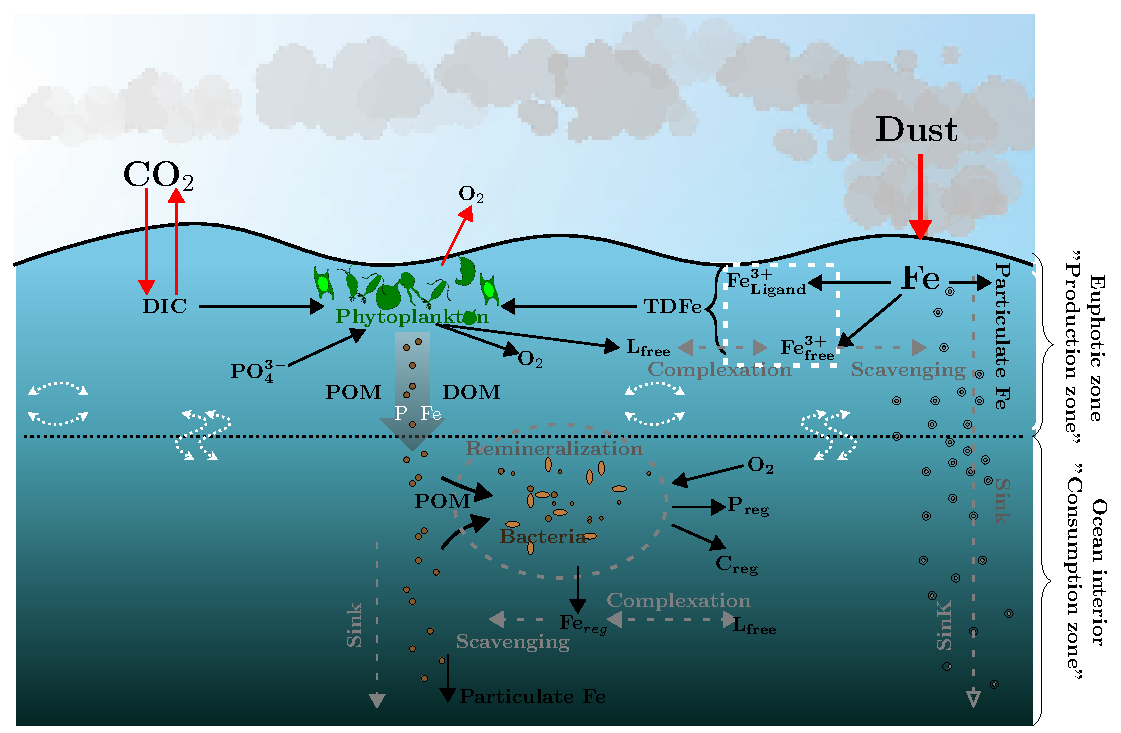
\includegraphics[scale=0.8]{../Paper_Draft/tikz/Fe.pdf}
    \caption{The iron (Fe) cycle in cGENIE. The only source of Fe to the ocean is dust. A fraction of supplied Fe will be complexed with organic ligands (Fe$^{3+}_{ligand}$), kept in free state (Fe$^{3+}_{free}$), and scavenged into particulate organic carbon (POC, Particulate Fe) to sink through the water column. The total dissolved Fe pool (TDFe) will be used by biology to generate particulate (POM) and dissolved (DOM) organic matter. The remineralization process will regenerate nutrients and carbon.}
\end{figure}

\subsection{General model description}

We use a version of the Grid-ENabled Integrated Earth (GENIE) model focused on the carbon (C) cycle, cGENIE muffin v0.9, with three modules: (1) the 3D frictional-geostrophic ocean module, with 16 depth levels and a 36x36 equal-area horizontal grid (constant 10° in longitude and uniform in the sine of latitude), (2) marine biogeochemistry module BIOGEM \cite{ridgwell2007marine}, and (3) an atmospheric component of the 2D energy-moisture balance model with prescribed climatological wind fields \cite{cao2009role}. The continental distribution and bathymetry are published in \citeA{ridgwell2007marine}.

For this study, we focused on the biological pump of soft tissues. For this purpose, a co-limitation scheme of iron (Fe) and phosphorus (P) to the C cycle was implemented following Tagliabue et al. (2016). Additionally, a simplified scheme of organic complexing, nutrient removal, and particulate organic C (POC) sink was implemented following the methodology proposed by \citeA{parekh2004modeling,parekh2006physical}. Table S1 in the Supporting Information summarizes the data sets and values used. The circulation model uses both parameterized temperature (van de Velde et al., 2021), salinity and 33 biogeochemical tracers to describe the interactions between nutrients. In order to make a correct C inventory, tracers and pre-formed nutrients were used following the base configuration of Cao et al. (2009).

In BIOGEM, C sequestration is controlled by biological export. The biogenic uptake of dissolved nutrients, tracers and inorganic C occurs in the ocean euphotic zone (upper 81 m). Remineralization by ocean bacteria (at a 590-m depth) results in dissolution (i.e., regeneration) of inorganic nutrients and C. Finally, the efficiency of the biological pump (P*) is defined in terms of the ratio of the regenerated (Preg) to total (Ptotal) P concentration: $P^{*} = P_{reg}/P_{total}$

\subsection{Model nutrient limitation scheme}

Both P and Fe have low ocean concentrations in many ocean basins, and in order to reproduce their limiting effects on primary productivity we use a colimitation scheme. The co-dependency between the concentration of dissolved phosphate ([PO$_4^{3-}$]) and the biological uptake of C at the surface ocean is expressed as:

\begin{linenomath*}
\begin{equation}
    P:C=1:\left(\frac{[PO_4^{3-}]}{144.9 \mu mol L^{-1}} + 0.006\right)^{-1}
\end{equation}
\end{linenomath*}

In cGENIE, the surface ocean is highly oxygenated and thus most of the Fe input is rapidly oxidized to Fe$^{3+}$ (Figure 2). Iron dissolution is a determining factor in photosynthesis and it will depend on water temperature, salinity, and pH. Total dissolved Fe (TDFe) will be composed of (1) free Fe (Fe$^{3+}_{free}$) and (2) ligand-bound Fe (Fe$^{3+}_{ligand}$). TDFe in the ocean is mostly present as  (~99\%), while Fe$^{3+}_{free}$ is the only species that is susceptible to be scavenged by POC and eliminated from the system when TDFe  is higher than the total concentration of ligands (L$_T$). In turn, L$_T$ consists of a free ligand component (L$_{free}$) and that associated to Fe (Fe$^{3+}_{ligand}$), and is invariant and uniform in the water column (0.1 nM) following Parekh et al. (2005) and Doney et al. (2006).

Finally, the Fe:C ratio is variable and parameterized to depend on TDFe, so that Fe requirements at the cellular level depend on Fe availability. Thus, under higher limitation, less Fe will be required and vice versa (a minimum ratio of 250,000 is imposed during maximum Fe limitation): 

\begin{linenomath*}
    \begin{equation}
Fe:c=\frac{1}{min(250,000,103,700 TDFe-0.4225)}
    \end{equation}
\end{linenomath*}

\subsection{Experimental design}

Six pairs of Holocene-Last Glacial Maximum (LGM) dust deposition rate fields were used as sources of soluble Fe to force cGENIE (for details see \citeA{lambert2021regional}. One of these pairs (Lambert) is derived from paleo-dust observations compiled by \citeA{lambert2015dust}, while the rest are derived from CMIP5 model simulations: Albani \cite{albani2014improved}, Takemura \cite{takemura2009simulation}, Ohgaito \cite{ohgaito2018effect}, MIROC-ESM \cite{sueyoshi2013set} and MRI-CGCM3 \cite{yukimoto2012new}. 

Since the solubility of iron in dust is not well known, a sensitivity analysis was carried out by creating different dust iron solubility fields for each dust deposition rate field. To achieve this, we start by deriving a field of fractional Fe solubility ($\Upsilon_{Fesol}$, \%) in dust based on each of the twelve dust deposition rate fields described in the previous paragraph (i.e., six for the Holocene and six for the LGM), calculated as: 

\begin{linenomath*}
    \begin{equation}
\Upsilon_{Fesol}= \gamma_{Fesol}C_{dust}^{-0.5}
    \end{equation}
\end{linenomath*}

where $\gamma_{Fesol}$ is a scaling factor and $C_{dust}$ is the concentration of dust in the surface ocean layer (see Text S1 of the Supplementary Information for further details). This relationship reflects observations that iron solubility of dust aerosols in weak acid solutions is inversely proportional to atmospheric dust load (Baker and Jickells, 2006).

Additionally, based on these twelve derived iron solubility reconstructions we created new fields by scaling all grid values by the same factor, as well as by scaling values of grid cells located within one of the five High-Nutrient, Low Chlorophyll (HNLC) ocean basins with respect to all other grid cells outside of any given HNLC ocean. In all cases the scaling factors used were 0.33, 0.67, 1.00 (i.e., no scaling factor applied), 2.00, and 3.00. Consequently, the model was forced with a total of 150 Holocene-LGM pairs of dust ($\Upsilon_{Fesol}$) fields. As we are interested in performing a sensitivity analysis of aeolian iron inputs to ocean CO$_2$ drawdown, all additional supplies of Fe associated with sedimentary processes in the ocean were not considered.

\subsection{Simulation}

\begin{figure}[h!]
    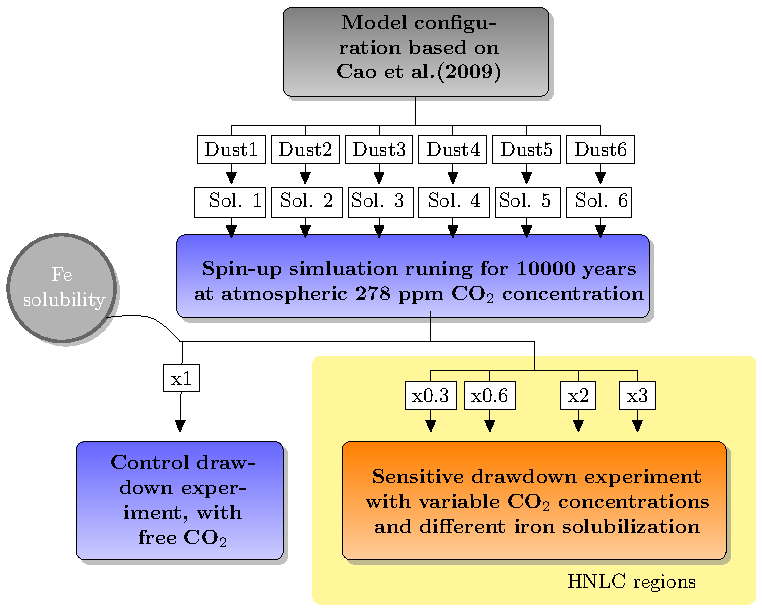
\includegraphics[scale=1]{../Paper_Draft/tikz/Figure3_diagram.tex.preview.pdf}
    \caption{Flow chart describing the experiment design. The gray box shows the general configuration used for spin-up and sensitivity experiment simulations. White boxes labeled Dust 1-6 represent the six Last Glacial Maximum (LGM) and six Holocene dust deposition flux fields used as input to the simulations, while the associated input fields of dust fractional iron (Fe) solubility are represented by white boxes labeled Sol. 1-6. The top blue box represents the spin-up simulations run for each input field of dust flux, using a fixed value for atmospheric carbon dioxide (CO$_2$) concentration. The bottom blue box represents the control simulations run with unprescribed CO2 for each input dust field (six for LGM and six for the Holocene). The bottom yellow box represents the main set of sensitivity experiment simulations, in which for all 12 input fields of dust fractional iron solubility, all grids of a given high-nutrient, low-chlorophyll (HNLC) ocean basin  are multiplied by the same scalar factor. }
\end{figure}

We spun up cGENIE by performing six different 10,000-year pre-industrial experiments in which atmospheric carbon dioxide (CO2) concentration was fixed at 278 ppmv (Figure 3). Each of these six simulations was forced by a Holocene dust ($\Upsilon_{Fesol}$) field. Starting from the end of each spin-up, we ran global and regional sensitivity experiments as described in the previous section for the Holocene and LGM, allowing the model to run for an extra 10,000 years. Finally, we took the mean of the last 500 years of CO2 concentration and carbon export rate from each simulation.


\section{Results}

% !TEX root = ../journaltemplate.tex

\subsection{Exploring Dust Iron Solubility}

\begin{figure}[h!]
    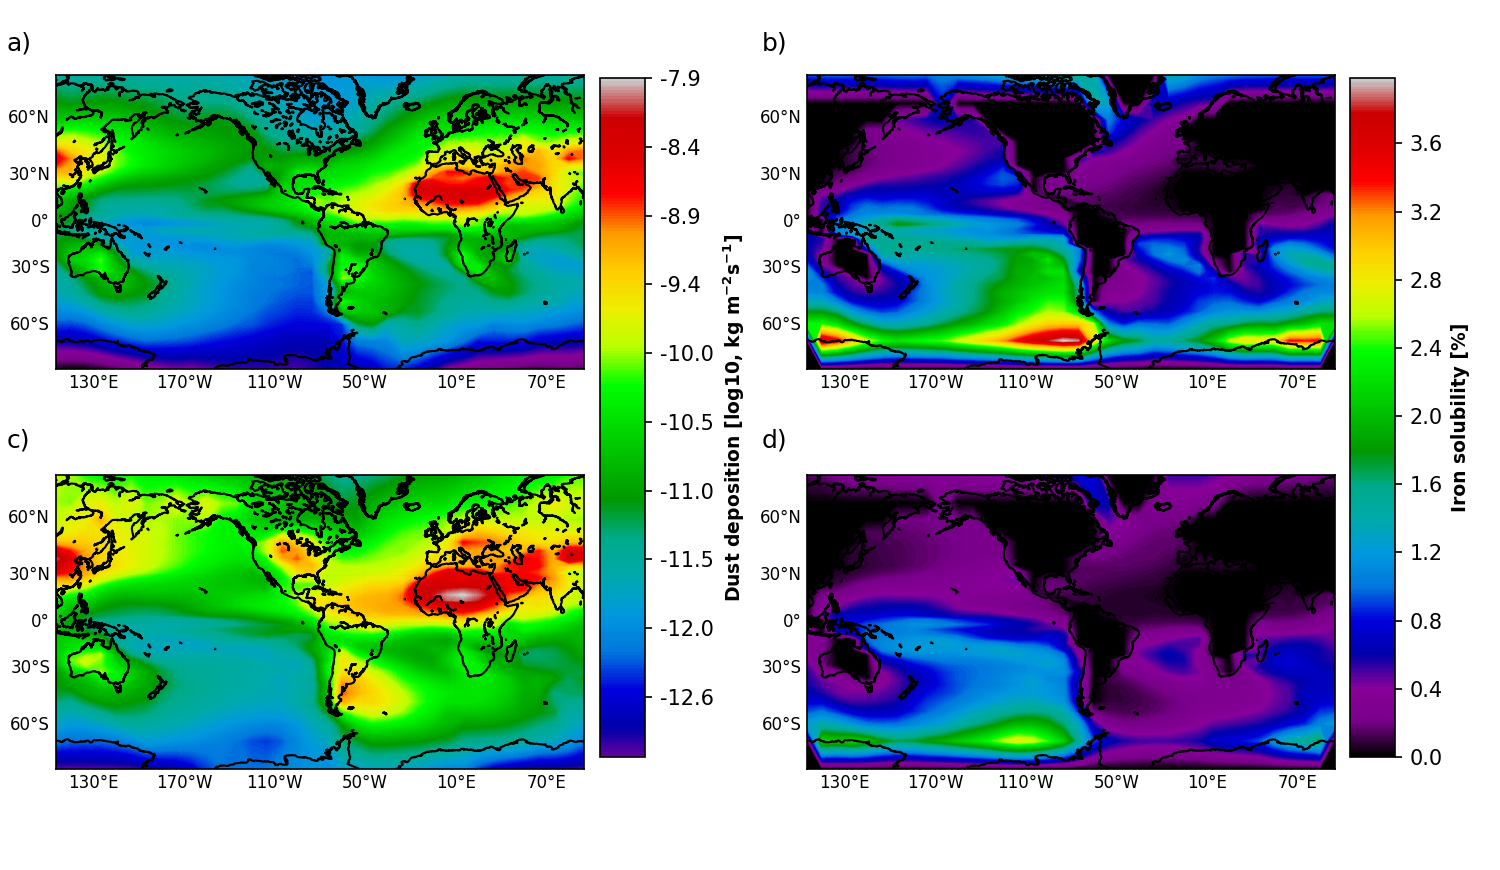
\includegraphics[scale=0.65]{../../Data_function/Function/PicturePaper/Figure7.png}
    \caption{Mean field of (a) Holocene and (c) Last Glacial Maximum (LGM) dust deposition rate derived from the six Holocene-LGM field pairs used in this study, and calculated fractional Fe solubility in deposited dust for the (b) Holocene and (d) LGM.}
\end{figure}


Figure 4 shows the mean fields of dust deposition rate considered in this study for the Holocene (Figure 4a) and LGM (Figure 4c), based on six Holocene-LGM pairs of individual fields as described in section 2.3, as well as the derived mean fields of $\Upsilon_{Fesol}$ in dust aerosols for the Holocene (Figure 4b) and LGM (Figure 4d). The latter constitute the base input fields of soluble Fe for our biogeochemical simulations. 

To properly interpret these results, it is important to clearly identify what processes of Fe solubilization are being captured by our methodology, and which are not. As was mentioned previously, the inverse relationship between $\Upsilon_{Fesol}$ in dust and atmospheric dust load used to derive our $\Upsilon_{Fesol}$ fields is based on laboratory Fe leaching experiments of aerosol samples collected over the ocean using a weakly acidic solution (Baker and Jickells, 2006). Under these conditions, Fe extracted into solution consists of a highly labile Fe fraction that may be extracted in pure water, and a water-insoluble fraction that is solubilized under weakly acidic conditions. Together, these two fractions constitute the so-called labile Fe (Perron et al., 2020). The highly labile fraction of Fe represents non-structural Fe adsorbed onto mineral surfaces, the so-called soluble Fe (Perron et al., 2020), so that leaching experiments performed with pure water (or seawater) mimic Fe solubilization during transport in non-acidic air masses (e.g., Chomchoei et al., 2005; Cosentino et al., 2020; Simonella et al., 2022). This Fe fraction may be considered the source-inherited Fe in dust, readily available without the need of atmospheric processing (Cosentino et al., 2020; Simonella et al., 2020). In turn, the water-insoluble, weak acid-soluble Fe represents structural Fe predominantly in clay minerals (Journet et al., 2008; Marcotte et al., 2020; Simonella et al., 2022), so that Fe leaching experiments with weak acids mimic proton-induced Fe processing during transport in acidic atmospheres (e.g., Cosentino et al., 2020; Simonella et al., 2022). Because soluble Fe is usually a small fraction of labile Fe, as low as 1\% even in close-to-source dust aerosols (e.g., Simonella et al., 2022), and because the relationship we used to derive our input $\Upsilon_{Fesol}$ fields represents labile Fe (Baker and Jickells, 2006), these fields mainly represent Fe solubility enhancement due to progressive fining of dust with greater distance traveled and associated rises in particle reactivity due to higher surface-to-volume ratios (Baker and Jickells, 2006; Cwiertny et al., 2008). Instead, our input fields do not capture differences in source-inherited Fe solubility of dust.


% Please add the following required packages to your document preamble:
% \usepackage{multirow}
\begin{table}[]
    \centering
    \begin{tabular}{||l|l|l|l|l|l|l||}
        \hline 
    \multirow{2}{*}{Model/Region} & \multirow{2}{*}{Global} & \multicolumn{5}{c}{HNLC ocean basin} \\
                                  &                         & NA    & NP    & CEP   & SP    & SAI  \\
    \hline \hline
    MMM\_PI                       & 0.65                    & 0.42  & 0.27  & 0.93  & 1.67  & 1.12 \\
    MMM\_LGM                      & 0.38                    & 0.21  & 0.13  & 0.62  & 1.10  & 0.59 \\
    Albani PI                     & 0.73                    & 0.34  & 0.23  & 0.60  & 1.86  & 1.13 \\
    Albani LGM                    & 0.27                    & 0.18  & 0.09  & 0.63  & 0.53  & 0.28 \\
    Lambert PI                    & 0.36                    & 0.30  & 0.15  & 0.66  & 0.51  & 0.68 \\
    Lambert LGM                   & 0.15                    & 0.12  & 0.06  & 0.35  & 0.20  & 0.44 \\
    Ohgaito PI                    & 0.99                    & 0.49  & 0.29  & 1.18  & 3.68  & 2.04 \\
    Ohgaito LGM                   & 0.35                    & 0.19  & 0.11  & 0.73  & 0.83  & 0.37 \\
    Takemura PI                   & 0.70                    & 0.51  & 0.41  & 0.96  & 1.50  & 1.32 \\
    Takemura LGM                  & 0.65                    & 0.31  & 0.31  & 0.62  & 1.47  & 1.63 \\
    MIROC-ESM PI                  & 0.77                    & 0.44  & 0.30  & 1.04  & 2.39  & 1.40 \\
    MIROC-ESM LGM                 & 0.76                    & 0.22  & 0.14  & 0.60  & 2.67  & 2.06 \\
    MRI-CGCM3 PI                  & 0.58                    & 0.38  & 0.23  & 1.06  & 1.44  & 0.85 \\
    MRI-CGCM3 LGM                 & 0.49                    & 0.29  & 0.16  & 0.89  & 1.44  & 0.70 \\
    \hline
    \end{tabular}
    \caption{Mean fractional iron solubility (\%) in deposited dust aerosols. NA: North Atlantic, NP: North Pacific, CEP: Central East Pacific, SP: South Pacific, SAI: South Atlantic and South Indian, PI: Pre-Industrial, LGM: Last Glacial Maximum. MMM: Multi-Model Mean}
    \end{table}

Table 1 illustrates the average global dust $\Upsilon_{Fesol}$ values for both the Holocene and the Last Glacial Maximum (LGM), alongside regional averages pertaining to the primary High Nutrient Low Chlorophyll (HNLC) ocean basins, considering the different dust fields employed in this study. Due to heightened dust loads during the LGM, dust $\Upsilon_{Fesol}$ reaches a global average of 0.38\%, notably lower than that of the Holocene (0.65\%). While the iron solubility (Fe) during dust transport is recognized to fluctuate up to 10\% with spatial heterogeneity (Journet et al., 2008), several studies adopt a fixed global measurement often below or near 1\% (Lambert et al., 2021; Odalen et al., 2020; Saini et al., 2022; Tagliabue et al., 2016).

The $\Upsilon_{Fesol}$ similarity between Takemura, and MIROC-ESM models is unsurprising, considering that both exclude glaciogenic origin dust source because used a similar aerosol module, while Ohgaito tend to underestimate the glaciogenic dust source originating from latitudes south of 30°S, thereby contributing to greater heterogeneity. The Lambert model displays the most pronounced deviation from the average; nevertheless, it demonstrates the most accurate representation of dust load for both North and South America, encompassing the sources of glaciogenic dust (Lambert et al. 2015).

On a regional scale, the Eastern Central Pacific (CEP), alongside the Southern Oceans (SO), South Pacific (SP), and South Indian Atlantic (SAI), exhibit the most pronounced dissolved iron inputs. Median values of 1.01\% (CEP), 1.71\% (SP), and 0.93\% (SAI) during the Holocene, and 0.62\% (CEP), 1.1\% (SP), and 0.43\% (SAI) during the LGM, respectively, are observed. As all models tend to proficiently replicate conditions in the CEP, it emerges as the region with the most adept concordance between models for both periods.

\subsection{Iron solubility effect on atmospheric carbon dioxide }

\begin{figure}[h!]
    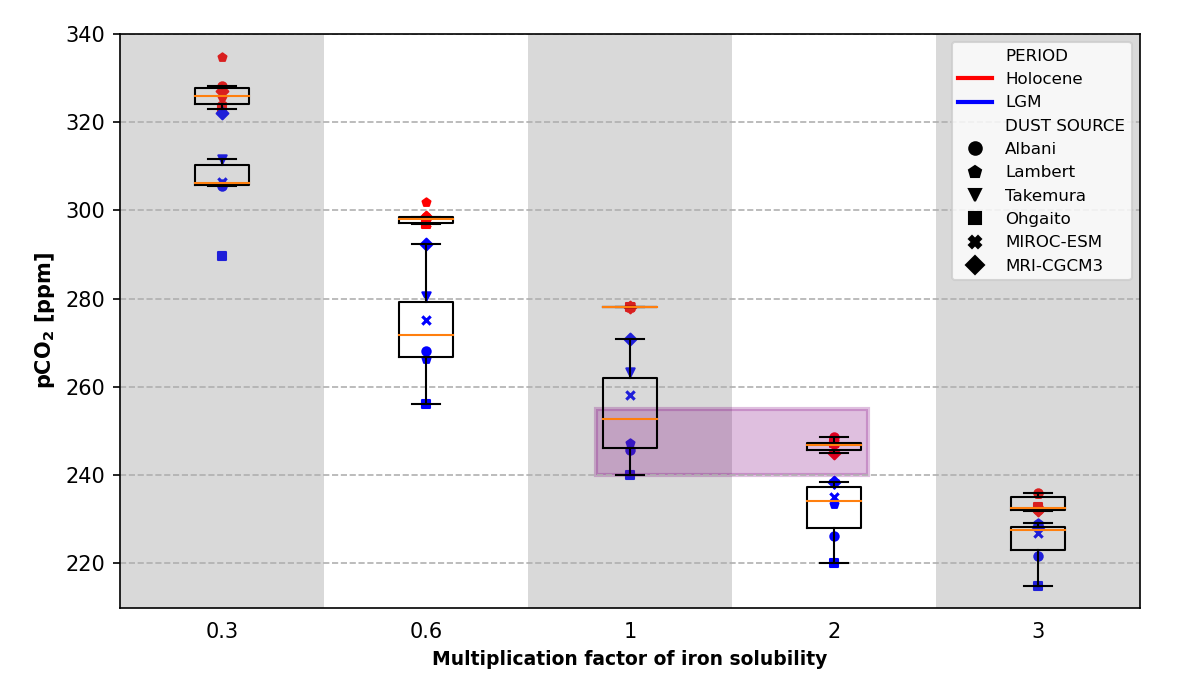
\includegraphics[scale=0.7]{../../Data_function/Function/PicturePaper/Figurex1_Subplot_CO2.png}
    \caption{Partial pressure of atmospheric carbon dioxide (pCO2) concentration for each experiment where iron solubility is multiplied by a factor between 0.3 and 3. Experiments using each of the dust deposition fields for Holocene (in red) and Last Glacial Maximum (LGM, in blue) are shown with different symbols.}
\end{figure} 

\note[N]{expandir caption Figure 4 para explicar los agregados de la figura: valores pCO2 de equilibrio}

As shown in Figure 5, increasing the solubility of Fe results in a decrease in atmospheric CO2 concentration. This relationship exhibits a marked non-linear behavior, suggesting a threshold for efficient Fe utilization, as also observed by Saini et al. (2022).  \annote[Naty]{This effect is also illustrated in Figure xx of the Supplementary Material, which shows that the Holocene and LGM experienced a maximum CO2 decrease of around 91 and 44 ppm, respectively. This finding indicates the point at which atmospheric CO2 concentration would experience no significant change due to the combined influence of dust and Fe solubility.}{Modificar figura original para que no haya suplementaria} 

Control simulations indicate that CO2 sequestration during the Holocene differs from that of the LGM. The variations in CO2 levels during glacial periods are between 7 to 37 ppm lower (Table 3), depending on the type of dust model and the Fe solubility associated with it. When bioavailable Fe levels increase, the difference in atmospheric CO2 between the LGM and Holocene is reduced (Figure 5). These findings suggest a potential buffering effect of Fe in the glacial ocean, which may become saturated more quickly due to the increase in dust flux during this period. 

The significant impact of Fe solubility on atmospheric CO2 capture is demonstrated by the rapid response of marine biomass. Our simulations show that doubling the Fe solubility of the Holocene triggers an average CO2 removal similar to that during the glacial period (see purple box in Figure 5), while tripling it results in a CO2 uptake equivalent to doubling the solubility during the LGM. In other words, doubling the current Fe solubility can lead to a global carbon sequestration comparable to the increase in dust during the last maximum glaciation. Our globally distributed dust fields exhibit LGM:Holocene ratios ranging from 1.4 to 4.7, which are consistent with other studies indicating 2.2 to 6.0 times pre-industrial concentrations (Albani et al., 2016: Lambert et al., 2015; Mahowald et al., 2006; Sudarchikova et al., 2015; Takemura et al., 2009). \annote[Naty]{We also found that at a certain point, when we quadruple the Fe solubility, the CO2 concentrations during both the Holocene and the LGM reach approximately 222 ppm (see Figure xx of the Supplementary Material)}{Sacar lo de figura suplementaria, cambiar por la figura 5}. This suggests that Fe solubility could play a key role in oceanic carbon fixation, which has been overlooked due to the scarcity of paleo-solubility data compared to Fe paleo-flux data. 

\subsection{Regional behavior}

\begin{figure}[h!]
    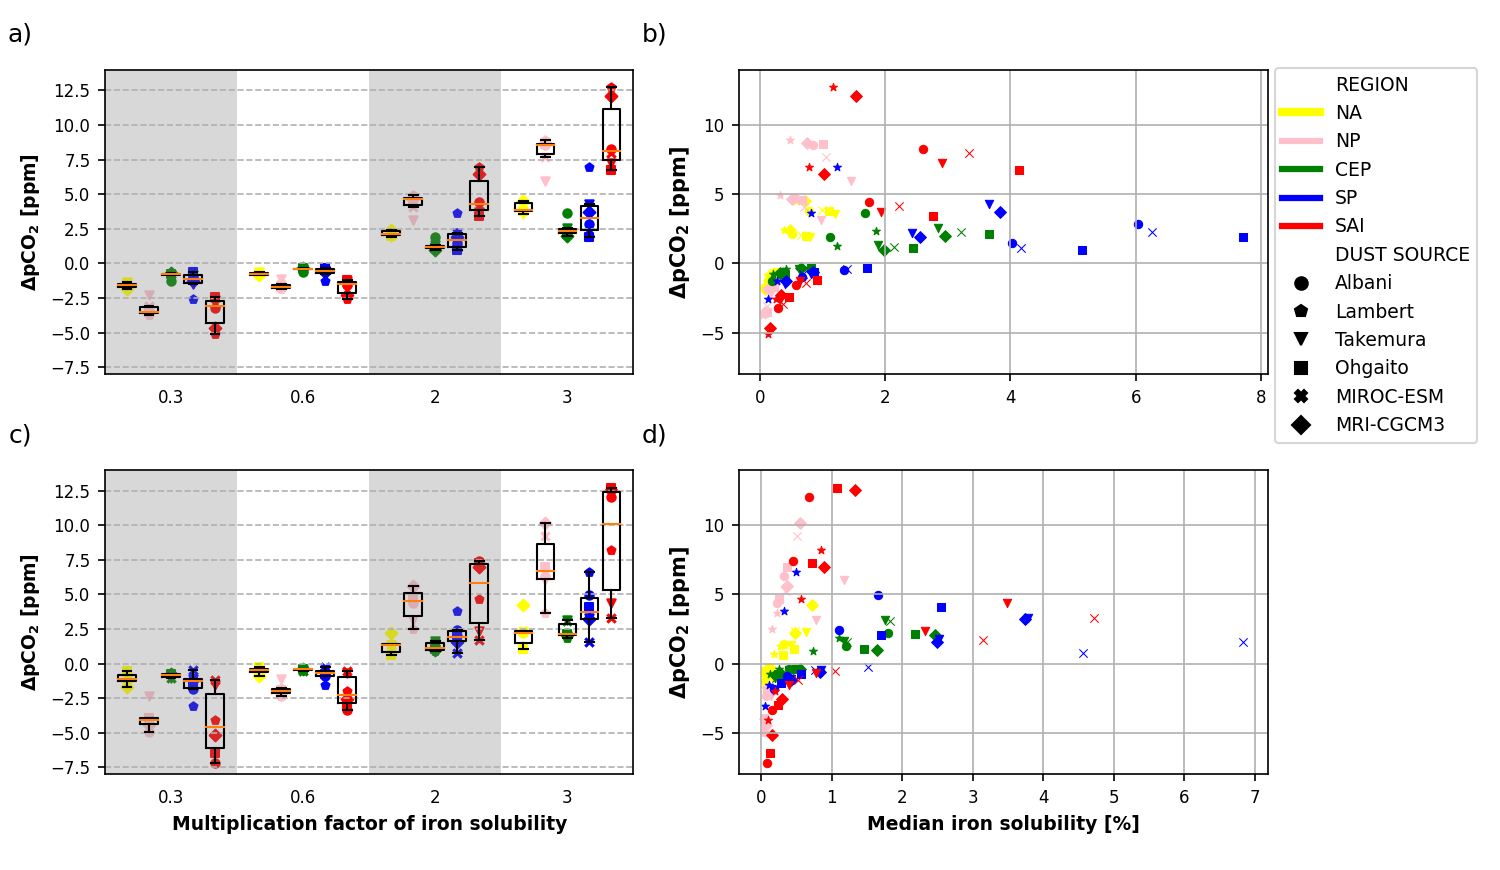
\includegraphics[scale=0.65]{../../Data_function/Function/PicturePaper/Figure4_Final.png}
    \caption{Difference in atmospheric carbon dioxide concentration ($\Delta pCO_2 = pCO_{2,control} - pCO_{2,experiment}$), for each experiment where iron solubility is multiplied by a factor between 0.3 and 3, compared to the same experiment with no factor applied (a and c). Experiments using each of the dust deposition fields for Holocene (a and b) and Last Glacial Maximum (c and d) are shown with different symbols. For each simulation (single data point), the factor of iron solubility was only applied to all grid cells within a specific high-nutrient, low- chlorophyll (HNLC) ocean basin (North Atlantic (NA), North Pacific (NP), Central Eastern Pacific (CEP), South Pacific (SP) and South Atlántic-Indian ocean (SAI)), while iron solubility in all other grid cells in the model was left unchanged. Results are also shown with respect to the median fractional iron solubility of the ocean basin considered (b and d). }
\end{figure}

In terms of regional patterns, our findings align with global trends. Increasing solubility above control levels results in higher CO2 sequestration (Figure 6a, 6c), and conversely. Sensitivity experiments to Fe variation show that during the LGM, CO2 concentration was reduced by 8-11\% above the capture of control simulations. The most significant variations occurred in the South Atlantic-Indian (SAI) region, where the maximum CO2 capture averaged 8.9 ppm. In the Holocene, although the regional patterns replicated those of the LGM, HNLC areas were responsible for a smaller proportion of global CO2 sequestration, accounting for only 44-62\% compared to 61-82\% during the LGM. This difference is likely due to lower dust deposition and a slight reduction in Fe solubility, particularly in HNLC regions relative to glacial periods (Figure 4b and 4d). During this time, the SAI region had an average maximum atmospheric CO2 capture of 9.2 ppm, while the North Atlantic basin became more active. 

Figure 6 illustrates how the Southern Oceans (SO), particularly the SAI basin, exerts a major control over CO2 sequestration, especially during the LGM, despite being highly sensitive to variations in Fe solubility (as shown in Figure 4b and 4d). This increase in sequestration during the LGM could be linked to elevated dust deposition in the region, which was significantly higher during glacial periods, reaching up to 20 times that of the Holocene (as reported by Lamy et al., 2014, and Dome Fuji Ice Core Project members, 2017). However, some models, such as MIROC-ESM and MRI-CGCM3,  tend to underestimate the magnitude of glaciogenic fluxes, possibly due to a lack of agreement in the way each model has been configured to represent vegetation distribution. The North Pacific (NP) basin is the second most active in terms of CO2 capture during both periods. These findings partially align with those of Lambert et al. (2021), with the main difference being observed in the Central-Eastern Pacific (CEP). Although it tends to differ slightly from control simulations in both periods, with maximum differences of 3 ppm for maximum solubility values, the North Atlantic (NA) appears to have the least impact on CO2 reduction during the LGM. Regardless of the Fe solubility value, the simulations show that the capacity to handle bioavailable Fe remains almost unchanged. However, during the Holocene, the CEP basin appears to play a more significant role than the South Pacific (SP) in terms of CO2 sequestration. This trend is possibly associated with weaker Fe deposition in the NA basin relative to the CEP, despite some models reporting increased fluxes from North Africa during the LGM. 

\subsection{Basin efficiency}

\begin{figure}[h!]
    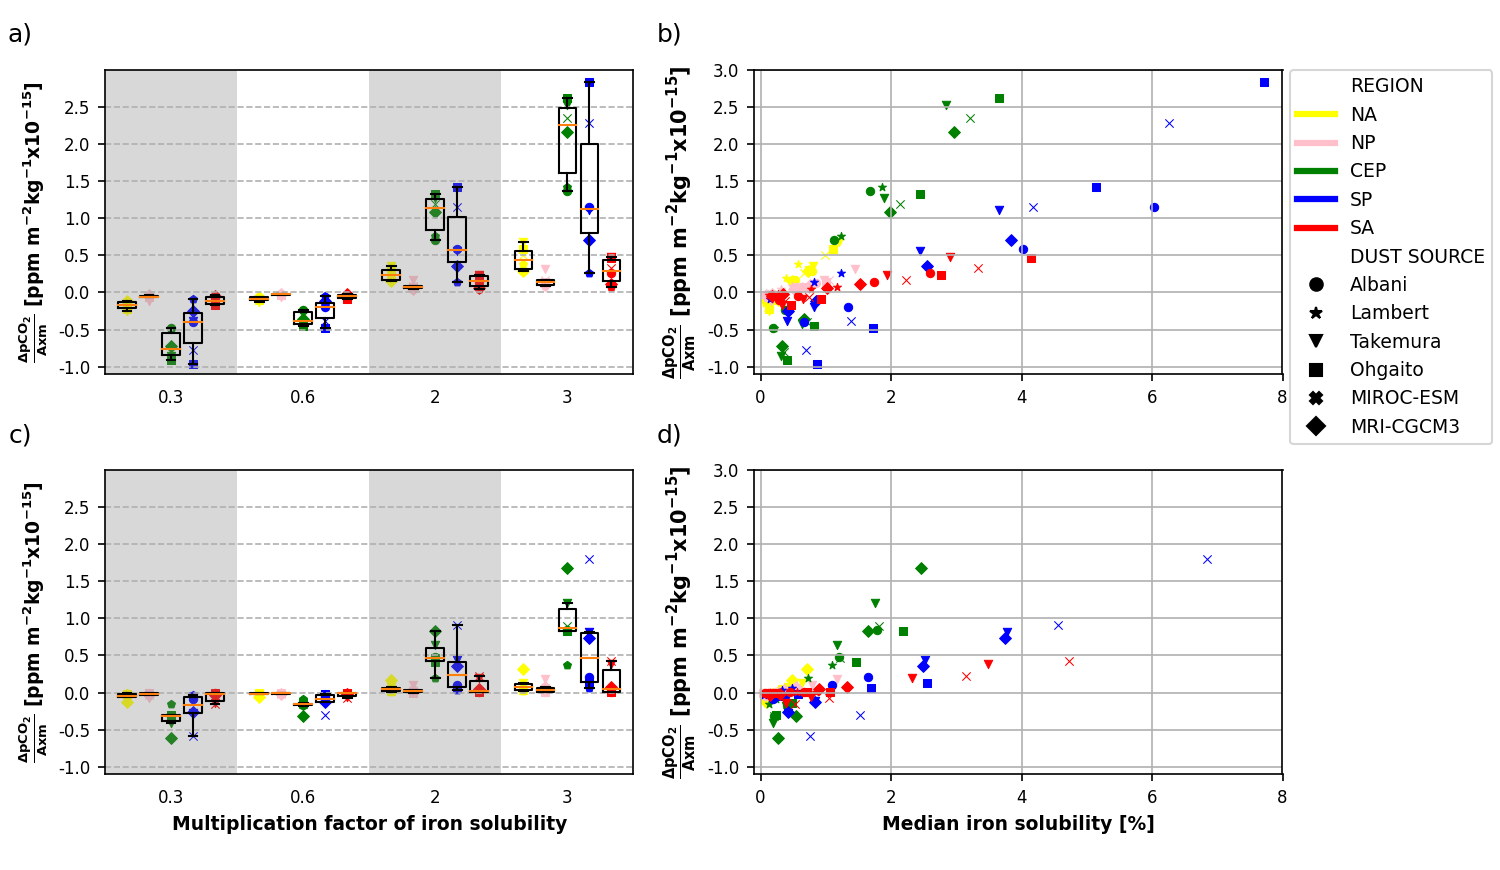
\includegraphics[scale=0.65]{../../Data_function/Function/PicturePaper/Figure6_Subplot_CO2Diff_Normalize.png}
    \caption{Difference in atmospheric carbon dioxide partial pressure (pCO$_2$) as in Figure 6, this time normalized by area and dust deposition load. }
\end{figure}

The contribution of different ocean basins to the total global CO2 reduction due to dust-borne Fe fertilization depends on both the total ocean basin area and the magnitude of iron deposition. When normalizing the CO2 concentration by both factors, it reveals that the SP and CEP basins are the most efficient in using available ocean resources to reduce atmospheric CO2 concentration for both periods (Figure 7). The CEP is an upwelling zone, therefore, a continuous nutrient supply makes this region of vital importance for the biological pump. However, when contrasting the Holocene and the LGM, we can see how the solubility of deposited Fe usually varies between 0.5 and 2.0\%, with lower values during the LGM (Figure 4b and 4d). These values are much lower than those found in the SP basin.  

There are remarkable hemispheric differences between basins (Figure 7b, 7d). While SO seems to display a \annote[N]{gradual}{creo que ac\'a "gradual" est\'a mal usado... discut\'amoslo el lunes} use of bioavailable Fe for CO2 capture, the rest of the HNLC zones show a tendency to be more efficient in utilizing deposited Fe. Therefore, with small amounts, they can achieve the same performance as large basins, as we can see by comparing the behavior of NP and SAI or CEP and SP. While these trends are evident in both periods, the hemispheric differentiation is more notable during the Holocene than during the LGM. The above more prominently demonstrates the saturation effect of Fe under higher rates of dust deposition. 

 


\section{Open Research}

\url{https://www.agu.org/Publish-with-AGU/Publish/Author-Resources/Data-and-Software-for-Authors#IGSN}
%%%%%%%%%%%%%%%%%%%%%%%%%%%%%%%%%%%%%%%%%%%%%%%

\acknowledgments
This section is optional. Include any Acknowledgments here.

%% ------------------------------------------------------------------------ %%
%% References and Citations


\bibliography{citas.bib} 

% don't specify bibliographystyle

% In the References section, cite the data/software described in the Availability Statement (this includes primary and processed data used for your research). For details on data/software citation as well as examples, see the Data & Software Citation section of the Data & Software for Authors guidance
% https://www.agu.org/Publish-with-AGU/Publish/Author-Resources/Data-and-Software-for-Authors#citation



%Reference citation instructions and examples:
%
% Please use ONLY \cite and \citeA for reference citations.
% \cite for parenthetical references
% ...as shown in recent studies (Simpson et al., 2019)
% \citeA for in-text citations
% ...Simpson et al. (2019) have shown...
%


\end{document}

%  To add line numbers to lines in equations:
%  \begin{linenomath*}
%  \begin{equation}
%  \end{equation}
%  \end{linenomath*}



